\documentclass{article}
\usepackage{polski}
\usepackage[utf8]{inputenc}
\usepackage[T1]{fontenc}
\usepackage{lmodern}
\usepackage[a4paper,top=2cm,bottom=2cm,left=3cm,right=3cm,marginparwidth=1.75cm]{geometry}
\usepackage{amsmath, amsfonts, amssymb, amsthm}
\usepackage{graphicx}
\usepackage{hyperref}
\usepackage{tcolorbox}
\usepackage{matlab-prettifier}
\usepackage{array}

\bibliographystyle{plain}

\title{Implementacja algorytmu mnożenia liczb dowolnej precyzji}
\author{Cybulski Mateusz, Derron Tomasz, Domiński Bartosz}
\date{}

\begin{document}
\maketitle

\begin{abstract}
    Implementacja algorytmu mnożenia Toom-Cook'a (Toom-3) dla liczb całkowitych dowolnej precyzji w C++. Zaprojektowanie i przeprowadzenie eksperymentu mającego na celu porównanie utworzonej implementacji z istniejącymi bibliotekami: GMP i wbudowaną biblioteką w Python.
\end{abstract}

\section{Metodologia}
\subsection{Cel eksperymentu}
Celem eksperymentu jest zbadanie zależności pomiędzy czasem wykonania operacji mnożenia a rozmiarem danych wejściowych dla utworzonej implementacji algorytmu mnożenia dużych liczb. W drugiej części eksperymentu, na podstawie otrzymanej zależności, nastąpi porównanie naszej implementacji z istniejącymi bibliotekami.
\subsection{Opis eksperymentu}
Zbiór liczb użyty w eksperymencie będzie skłądał się z liczb w zapisie o podstawie $\beta=2^{32}$. W eksperymencie zostaną użyte liczby z zakresu od liczb 50-słowowych do 1000-słowowych (zakładamy, że słowo = 32 bity).

Będziemy mierzyć czas wykonania operacji mnożenia dla liczb o długości 50, 100, 150, ... , 950, 1000 słów. Dla każdej z podanych długości zostanie wygenerowanych 100 liczb o zadanej długości, następnie w pseudolosowy sposób zostaną dobrane w pary, i na tych parach (50 par dla każdej z ustalonych długości) zostanie przeprowadzone mnożenie. Zakres długości liczb został wybrany na podstawie wykresu \cite{BrentZimmermann2010}, pokazanego poniżej.

\begin{figure}[h]
    \centering
    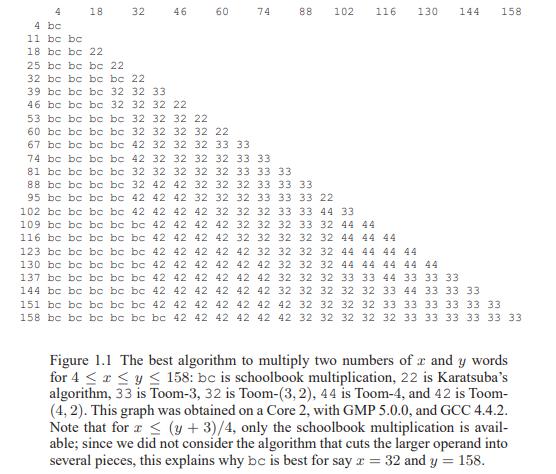
\includegraphics[width=0.5\linewidth]{wykres_wybór_algorytmu.png}
    \caption{Algorytm mnożenia stosowany w zależności od długości słów.}
    \label{fig:placeholder}
\end{figure}

Do wygenerowania pseudolosowych liczb jako próbek o zadanej długości zostanie użyty moduł \textit{random}.

Następnie zostanie zbadana zależoność czasu potrzebnego do przeprowadzenia operacji mnożenia w zależności od tego jak duże są mnożone liczby dla utworzonej przez nas implementacji.

Następnie te same pary liczb zostaną pomnożone z wykorzystaniem biblioteki GMP (GNU Multiple Precision Arithmetic Library) oraz w języku Python. Umożliwi to wyznaczenie analogicznej zależności jak dla naszej implementacji, oraz ich porównanie.

\subsection{Plan osiągnięcia celów projektowych}
\bigskip
\noindent \textbf{Szkielet implementacji}

\begin{itemize}
    \item Fork szkieletu implementacji -- znalezienie dostępnego rozwiązania i wykorzystanie go zgodnie z licencją.
    \item Edycja kodu -- usunięcie zbędnego kodu, zmodyfikowanie pod własne potrzeby.
\end{itemize}

\bigskip
\noindent \textbf{Implementacja dodawania BigInt}

\begin{itemize}
    \item Algorytm dodawania -- niezbędny do poprawnego działania mnożenia.
    \item Testy poprawności -- weryfikacja wyników.
\end{itemize}

\bigskip
\noindent\textbf{Algorytm mnożenia}

\begin{itemize}
    \item Implementacja Toom-3 -- wykorzystując wcześniejszy szkielet.
    \item Testy poprawności -- porównanie wyników z bibliotekami.
\end{itemize}

\bigskip
\noindent\textbf{Eksperyment i benchmarki}

\begin{itemize}
    \item Przygotowanie próbek -- z użyciem gotowej biblioteki do generowania liczb pseudolosowych i zapis danych wejściowych według ustalonej metodologii.
    \item Testy własnej implementacji -- pomiar czasu mnożenia próbek.
    \item Testy rozwiązań GMP -- benchmark względem profesjonalnego standardu C++.
    \item Testy rozwiązań wbudowanych w Pythonie -- pomiar czasu w Pythonie.
    \item Zapisanie wyników -- względem ustalonej metodologii (.csv).
\end{itemize}

\bigskip
\noindent\textbf{Analiza wyników}

\begin{itemize}
    \item Wykresy i analiza danych -- wykorzystanie bibliotek Python.
    \item Wnioski końcowe -- podsumowanie efektywności algorytmu w praktyce.
\end{itemize}

\newpage
\bibliography{references}

\end{document}
